\title{Rhizosphere metagenomics of three biofuel crops}
\author{}

\documentclass[12pt]{article}
\usepackage[a4paper, margin=1in]{geometry}
\usepackage[parfill]{parskip}

% set double space
\usepackage{setspace}
\doublespacing

% set times fond
\usepackage{times}

% line number index
\usepackage{lineno}
\linenumbers

% Compile only with pdfLaTeX
\usepackage[pdftex]{graphicx}

% nice table format
\usepackage{booktabs}

% caption adjustment
\usepackage{caption}
\captionsetup[table]{singlelinecheck=off}

\begin{document}
\maketitle
\section{Introduction}

- Bioenergy and sustainability

Bioenergy is green energy, but growing bioenergy crop is not fully environmental friendly. With appropriate management, it can however be managed to have positive environmental effects. One area of management where sustainable development could help increase benefits is the growth of bioenergy crops. Bioenergy crop growth requires energy inputs (fertilizer, pesticides for corn), emits greenhouse gases (CO2, N2O), and competes with food production for land 1. The rhizosphere, or the interface between plant roots and soils, is an especially important part of the soil where microbes and plants form beneficial associations. Rhizosphere microbes provide critical nutrients (N, P) to plants, produce hormones that promote plant growth, improve plant pathogen resistance, and improve the soil physical structure in addition to many yet unknown beneficial relationships 2–6. This beneficial supporting microbial community is important for sustainable plant growth and consequently identifying these beneficial microbes and their functions is important for low cost growth of bioenergy plants.

- Three crops, annual and perennial, agricultural management

Rhizosphere microbes are influenced by many factors, such as the particular vegetation, agricultural management inputs, soil type, moisture and other environmental factors. In several large-scale studies, microbial communities are usually clustered based on their location because soil and ecosystem type has long-term selection and thus stronger influence than other factors. Vegetation also has influence on microbial community structure through the root exudates and particulate residues, which is the primary annual carbon and energy source for soil microbes. However, their influence varies depending on the plant species and ecosystem type 7,9,10. Three biofuel crops (corn, switchgrass and miscanthus) are from the same family (true grasses), but they are very different in phenotype. Miscanthus and switchgrass are perennial grasses with fibrous roots, while corn is an annual with less fibrous root. Miscanthus is the largest in size and originated from tropical regions, while switchgrass is native in Midwest, US. Large scale planting of these biofuel crops may impact soil microbial community structure and function, including N cycle processes. Plants also take time to select their beneficial groups and stabilize them, so the time since the establishment is also an important factor. Since switchgrass and miscanthus can growth with no (or less) new N input 7,11, these two perennial grasses are thought to have better nitrogen sustainability. Moreover, miscanthus is big in size and thus thought to have a community more efficient at fixing and keeping nitrogen in the soil. My preliminary studies have shown that the corn selected community is more different from switchgrass and miscanthus, than the later are from each other. However, it is still not clear which microbial groups make the miscanthus rhizosphere microbial community more efficient with its N economy 11,12.

Other than vegetation, agricultural management of the vegetation such as tillage, liming, and fertilization, also influence the rhizosphere microbial community by changing soil physical and chemical characteristics 13,14. Application of nitrogen fertilizer should decrease N fixation and increase nitrification and denitrification because N fixing microbes are not selected in higher N environments while nitrifying and denitrifying bacteria should be favored since they have more substrate. Within the nitrifying community, AOB (ammonia-oxidizing bacteria) is more responsive to fertilization than AOA (ammonia- oxidizing archaea), though AOA is usually more abundant than AOB 8,15. In the management of these three biofuel crops, corn needs more nitrogen fertilizer while switchgrass and miscanthus needs very little. Nitrogen fixing microbes may play an important role providing nitrogen for growth of miscanthus. Previous studies have shown that sugarcane can have 40\% to 60\% of its nitrogen supply from bacterial nitrogen fixation 16,17. Thus miscanthus and corn, close relatives of sugarcane may also enrich nitrogen fixing bacteria. Another study based on amplicon sequencing and qPCR of a few N-cycle genes found the abundance of N-fixing genes (nifH) is significantly higher in miscanthus and switchgrass than corn 7. The microbial communities of miscanthus and switchgrass are adapted to a low N environment and more efficient at keeping nitrogen in the soil, so are predicted to have increased N fixation, and decreased nitrification and denitrification. In addition, species well adapted to low the N environment should increase.

In addition to fertilization, the difference on the ways these three crops re-grow may also make a difference in their microbial community. Corn re-grows from new seeds, while the two perennial grasses continue to grow from their existing crown/roots. I predict that corn will select the fast growers since they grow a new root system and select its rhizosphere community every year. The perennial should have a more stable rhizosphere community because the selected community from previous year is less disrupted.

- N cycle

Despite the limited understanding of rhizosphere microorganisms, the chemistry of the nutrient cycles carried out by those microorganisms is relatively clear, including nitrogen fixation, nitrification, and denitrification. Nitrogen fixing microbial community are commonly measured with nifH as marker and nitrifying community are commonly measured with AOA (archaeal amoA) and AOB (baterial amoA). Denitrification has multiple steps including nitrate reduction (Nar), nitrite reduction (Nir), nitric oxide reduction (Nor) and nitrous oxide reduction (Nos). Denitrifying community are commonly measured with Nir, Nor, and Nos. Nir has two types, Cu-Nir (copper based) and cd1-Nir (iron based), encoded by nirK and nirS respectively. Nor has cNor (with cytochrome c) and qNor (without cytochrome c). Nos also has two types, encoded by typical nosZ and atypical nosZ. Studies only survey one gene may underestimate microbes involved in denitrification. (ADD REF)

- Amplicon vs. shotgun metaG

Many previous studies have focused on identifying N-relevant genes in soils through PCR-amplified amplicons of targeted genes (SSU rRNA gene or N cycle genes) 7,12. However, primer bias is a well-known problem for amplicon-based analysis, especially for those N cycle genes that lack well curated reference databases 18–20. Here, I propose to use high throughput shotgun sequencing provided by Illumina Hiseq technology. All DNA in the community is randomly fragmented and sequenced to produce less biased metagenomes of microbial communities compared to gene-targeted amplicons. Further, rather than amplicons only targeting one gene or part of a gene, the shotgun method produces short fragments representing entire genomes. Thus, the shotgun method produces potentially all the genetic information of community members. The challenge to using the shotgun approach is that its analysis is challenging due to its big data size and short read lengths. To answer my research questions, our group have developed efficient methods to assemble metagenome and also extract genes of interest in the big soil shotgun sequencing data (ADD REF, SSUsearch, dignorm+partition, Xander).

Other than using better sequencing technology, we sampled the rhizosphere very close (on the roots or associated soil fragments, {\textless} 2 mm) to the roots rather than bulk soil as used in other studies 7. Similar rhizosphere sampling methods have been use in some studies 23,24. Even though bulk soil community is also influenced by the plant roots, they are more influenced by soil physical and chemical characteristics and long history of agriculture management. Rhizosphere, as the interface of soil and plant roots, is more impacted by the plant roots so better represents the selection effects of the plant. This rhizosphere sampling method better serves our goals to find the groups and genes selected by plants.

\section{Methods}

{\bf Soil samples, DNA extraction, and sequencing.}
Rhizosphere samples of corn, switchgrass and Miscanthus were collected at Great Lake Bioenergy Research Center (GLBRC) intensive Cropping System Comparison site in Kellog Biological Station (KBS) (N:xx, W:yy) in Michigan on 10/12/2012, http://data.sustainability.glbrc.org/pages/1.html. We sampled rhizospheres of each crop at seven plot areas. Each replicate was a composite of two or three plant close to the sampling spot. Roots were shaken vigorously to remove loosely attached soil, then cut off from stem and placed in plastic bags 4 degrees C. Soil closely attached to roots ({\textless} 1 mm) were collected as rhizosphere soil in lab (details see add ref Ederson). Soil left in plastic were send to measure soil chemistry. DNA was extracted with PowerSoil DNA Isolation Kit from MO BIO, USA (details see add ref Edersion) and then sent to Joint Genome Institute (JGI) for Illumina HiSeq 2500 sequencing (250 bp insert libraries and 2 x 150 bp reads).

{\bf Data preprocessing.}
Raw Illumina reads were quality trimmed using fastq-mcf (version x.x.x, http://code.google.com/p/ea-utils) with flags ``-l 50 -q 30 -w 4 -x 10 --max-ns 0 -X''. Then paired ends were merged by FLASH (add ref) using flags ``-m 10 -M 120 -x 0.20 -r 140 -f 250 -s 25''.

{\bf Diversity analysis using SSU rRNA gene.}
SSU rRNA gene fragments in shotgun metagenome are identified and an OTU table was made using fragments aligned to a 150 bp region of V4 (E.coli position: xx - yy) by SSUsearch pipeline (add ref). Ordination, richness and diversity analysis were calculated by phyloseq and vegan package in R (add ref). Venn diagram were made by in house python scripts.

{\bf Global metagenome assembly, annotation and functional diversity.}
Preprocessed reads of each crop were pooled and then assembled with digital normalization (-C 10) and partitioning pipeline (add ref) following tutorial provided in xxxx with khmer (version xx). The partitioned data were then assembled with velvet (version xx) (add ref) and SGA (version xx) (add ref). For velvet, kmer size of 29, 39, 49, 59 and 69 were used and final assembly was merged with SGA. For SGA, overlap size of 29, 39, 49, 59, and 69 were used and final assembly were clustered using cd-hit-est (-c 0.99) in CDHIT (add ref). Contigs shorter than 300 bp were discarded. Since velvet and SGA produced very similar assembly in terms of total size and longest contigs. The assembly from SGA was chosen for further analysis.

The assembly was then uploaded to MG-RAST (add ref) for gene calling and annotation. Gene calling files (with suffix .genecalling.coding.faa), clustering files (with suffix .cluster.aa90.mapping), and BLAT (add ref) tabular output files (with suffix .superblat.sims) were downloaded. BLAT hits with alignment longer than 30 amino acids, identity higher than 70\%, and E-value lower than 0.00001 were used for downstream analysis. Number of hits to each reference in MG-RAST M5NR database for each sample was summarized based on BLAT hits, gene calling IDs, and clustering info. Then M5NR IDs were converted into subsystem IDs and further subsystem ontologies using MG-RAST API (http://api.metagenomics.anl.gov/api.html). At the end, an count table of subsystem ontologies across each samples was made. Level 3 and Level 1 subsystem were used for ordination analysis with R phyloseq package (add ref). For enrichment analysis, group\_significance.py in QIIME was used to find level 3 subsystems (pathways) that significantly different between two crops ($p < 0.05, n = 7$) and those pathways with more than 10 total counts in all samples and a fold change less than 0.5 or larger than 2 were treated as significant.

{\bf N cycle gene assembly and diversity.}
Preprocessed reads of each crop were used as input to Xander (gene targeted metagenomic assembler) (add ref) with MAX\_JVM\_HEAP=300G, FILTER\_SIZE=40, K\_SIZE=45, genes=''nosZ nosZ\_a1 nosZ\_a2 nirS amoA\_AOA amoA\_AOB norB\_cNor norB\_qNor narG''. Output files with taxon abundance (``*\_taxonabund.txt'') were used for taxonomy based analysis. The abundance of each N cycle genes were normalized by number of rplB gene (single copy gene). In OTU based analysis, assembled gene sequences are clustered by McClust (add ref), mean coverage in ``*\_coverage.txt'' were used to adjust abundance of each OTU, and diversity analysis was done by vegan package in R.

{\bf Reproducibility and data accession.}
The scripts used to analyze the data are available at GitHub. Raw reads can be accessed at JGI portal with accession number: xx, yy, and zz. Assembled contigs can be accessed at MG-RAST at xx, yy, and zz.

\section{Results}

1) SSU
- beta-diversity: venn, pcoa
  - PCoA
  - shared OTU w/ and w/o weighing abundance
  - best match genus

The average read number after quality trimming and pair end assembly was about 228 millions (range from 140 millions to 285 millions) for each replicate. The reads sizes range from 50 bp to 290 bp. An average of 0.039\% of data were identified as SSU rRNA gene fragment (Table X). The number of SSU rRNA gene fragments aligned to 150 bp of V4 region is 9.4\% on average (range from 8.3\% to 10.0\%).

All samples were subsampled to the same number (4598) of SSU rRNA gene fragments and a total of 12841 OTUs are clusted. The OTU number in each replicate is 2164 on average (range from 1707 to 2355, Table X).

Ordination analysis using OTUs clustered from fragments aligned to V4 region of SSU rRNA gene showed that perennial grass (switchgrass and Miscanthus) had significantly different community structure from annual grass (corn) (AMOVA test: $p < 0.001$). The variation between corn and perennials is on PC1 and PC1 took up 48\% of total variation. Difference between Miscanthus and switchgrass were not significant and mainly varied on PC2 that only took up 8\% of total variation (Fig.~\ref{fig:otu-pcoa}). Corn also had greater dispersion than the perennials. Venn diagrams were used to quantify similarity among communities. Three crops shared 21.5\% of their total unique OTUs, but 73.1\% of all members when abundance of each OTU was considered. At genus level, they shared 55.2\% of unique genera, but 98.1\% of all members when abundance of each genus was considered. @add anosim analysis.

- richness, diversity, evenness

Microbial community in perennials rhizosphere have higher species richness (ACE) and diversity (inverse simpson) than in corn (Fig.~\ref{fig:otu-alpha-div}). Members in perennials are also more evenly distributed than in corn (Fig.~\ref{fig:otu-rankabuncurve}).

Corn had more Proteobacteria in rhizosphere while perennials had more Acidobacteria. Proteobacteria are mostly faster growers and Acidobacteria are mostly slow growers (add ref). Thus corn selected for faster grower while perenials selected for slow growers. Top three genera are Sphingomonas (Proteobacteria), Penicillium (Fungi), Burkholderia (Proteobacteria) in corn, Da023 (Acidobacteria), Akiw534 (Actinobacteria), Sphingomonas (proteobacteria) in Miscanthus and switchgrass.

- domain distribution (fungi, Table X) (discuss the C/N ratio, AMF --> corn does not have control ).

Bacteria, Archaea, and Eukaryota were 91.9\%, 0.7\%, and 7.2\% respectively on average across all samples (Table X). Corn (4.9\%) had more fungi than Miscanthus (2.2\%) and switchgrass (2.0\%). However, relative abundance of AMF (Arbuscular Mycorrhizal Fungi) was lower in corn (0.1\%) than Miscanthus (0.3\%) and switchgrass (0.4\%).
  
2) Global assembly

- computation time

We applied digital normalization and partitioning method (ADD REF) to assemble pooled data (300 Gb) for each plant. The average computation time is 1510 cpu hours (63 days in total, Diginorm: 71h, Filterbelow: 25h, Loadgraph: 1166h, Partgraph: 205h, Mergegraph: 8h, Annograph: 27h, Extrgraph: 8h). Memory usage varies in difference steps. The peak memories used is 1 TB in digital normalization, which produced an average false positive rate of XX in kmer counting and false positive rates below 20\% are acceptable for digital normalization(ADD REF). 

- assembly stats

Our assembly method produced  6.4, 6.0 and 5.3 Gb assembly with median contig size of 400, 391, 391 bp and maximum contig size of 21.0, 15.7, 16.0 kbp for corn, Miscanthus, and switchgrass respectively (Minumum contig size cutoff: 300 bp)(Table X). When mapping quality trimmed reads to assembly, we found 20.7\%, 19.1\%, and 20.3\% reads could be mapped (Table X). The read mapping back rate suggested percentage of trimmed read data assembled.

- contig comparison @check effect of different size cutoff

We also compared three biofuel crops based on sequence similarity among assemblies. Corn was the most different among three biofuel crops. Corn and Miscanthus shared 17\% of assembled contigs, corn and switchgrass shared 17\%, and switchgrass and Miscanthus shared 26\%.

3) Functional annotation from assembly

- PCoA with functional categories

After the assembled sequences were annotated by MG-RAST, we used ``Subsystem'' annotation for further analysis. Ordination analysis with both subsystem level 1 and 3 showed corn was different perennials and no significant difference between Miscanthus and switchgrass. The total variation explained by first two PCs are XX \% and YY \% in PCoA with level 1 subsystems and XX \% and YY \% in PCoA with level 3 subsystems (Fig.~\ref{fig:subsys-l1-pcoa},\ref{fig:subsys-l3-pcoa}). @ add anosim analysis.

- DE analysis with corn and Miscanthus
Since the above ordination analysis showed corn was the most different, we picked Miscanthu as an representative of perennials and focus on the comparison between corn and Miscanthus. Using level 1 subsystems, we found rhizosphere of corn was enriched in ``Iron acquisition and metabolism'', ``Membrane Transport'', ``Cell Wall and Capsule'', ``Phages, Prophages, Transposable elements, Plasmids'', ``Motility and Chemotaxis'', and ``Carbohydrate'', while Miscanthus was enriched in ``Amino Acids and Derivatives'', ``Cell Division and Cell Cycle'', ``Nucleosides and Nucleotides'', ``Protein Metabolism'', ``RNA Metabolism'', ``Secondary Metabolism'', ``Potassium metabolism'', ``Respiration'', ``Photosynthesis'', ``Regulation and Cell signaling'', and ``Stress Response'' (FDR adjusted p < 0.05, n = 7).

We also used level 3 subsystems (pathway) and found corn had more pathways significantly enriched belonging to level 1 subsystems of ``Stress Response'', ``Carbohydrate'', and ``Cell Wall/Capsule'', while Miscanthus had more pathways significantly enriched in ``Amino Acids and Derivatives'', and ``Respiration''.

Within ``Stress response'', ``Desiccation stress'' and  ``Oxidative stress'' were significantly higher in corn, while ``Cold shock'' and ``Osmotic stress'' were significantly higher in Miscanthus. Within ``Carbohydrates'', ``Sugar alcohols'', ``Aminosugars'', and ``Monosaccharides'' were enriched in corn, while ``CO2 fixation'', ``Central carbohydrate metabolism'', and ``Polysaccharides'' were enriched in Miscanthus. Within ``Phages, Prophages, Transposable elements, Plasmids'', ``Gene Transfer Agent (GTA)'', ``Plasmid related functions'', and ``Phages and prophages'' were enriched in corn, while ``Transposable elements'' were enriched in Miscanthus. Within ``Nitrogen Metabolism'', ``Nitrilase'' and ``Cyanate hydrosis'' were enriched in corn, while ``Dissimilatory nitrate reductase'', and ``Denitrification'', ``Allantoin Utilization'', ``Nitrogen Fixation''  were enriched in Miscanthus (FDR adjusted p < 0.05, n = 7).

4) Xander assembly results

- N cycle gene abundance and taxonomy composition.

We used Xander (ref), a gene targeted assembler, to assemble the N cycle genes for further diversity analysis of this functionally important group.

N cycle genes abundances, including nitrogen fixation genes (nifH), nitrification genes (AOA and AOB), and denitrification genes (nirK, nirS, nosZ, nosZa2, qNOR, and cNOR) normalized by rplB abundance were shown in Figure ~\ref{fig:xander-ncycle-abun}. NifH, AOB, nirK, nosZa2, and qNOR were significantly different between corn and Miscanthus. NirK, nosZ and qNOR  were significantly different between corn and switchgrass. AOA and nosZ was significantly different between Miscanthus and switchgrass ($p < 0.05, n = 7$).

When combining the genes with the same function, nitrite reductase genes (nirK and nirS) are significantly more abundant in corn, but nitric oxide reductase genes (qNOR and cNOR) and nitrous oxide reductase genes (nosZ and nosZa2) are significantly more abundant in perennials.

- ratios of interest
We also look at the ratio of nitrification/fixation (amoA/nifH) and denitrification/nitrification (nirK+nirS/amoA, qNor+cNor/amoA, and nosZ+nosZ/amoA). There were no significantly difference among three crops for all the above ratios ($p < 0.05, n = 7$). However, the median of amoA/nifH is the highest in corn. The median of nirK+nirS/amoA, qNor+cNor/amoA, and nosZ+nosZ/amoA are all highest in switchgrass.

There are several pairs of genes coding for enzyme of the same process and we found a consistent pattern across all samples: AOA {\textgreater} AOB, nirK {\textgreater} nirS, nosZa2 {\textgreater} nosZ, qNOR {\textgreater} cNOR (Fig.X,Y). Moreover, nitrification gene abundances (AOA and AOB) were higher than nitrogen fixation genes (nifH), and denitrification gene abundances (nirK and nirS, qNOR and cNOR, or nosZ and nosZa2) were higher than nitrification genes (AOA and AOB) (Fig.X).

%add alpha diversity with taxon table?
We also looked at detailed genus level distribution of nifH. There were 7, 9, and 5 genera in corn, Miscanthus, and switchgrass, respectively. The taxonomic composition of the communities were different among three crops. On average, Rhizobium, Bradyrhizobium, and Methylobacterium were the most abundant in corn, Coraliomargarita, Azospirillum, and Nostoc were the most abundant in Miscanthus, and Novosphigobium, Gluconacetobacter, and Azospirillum were the most abundant in switchgrass (Figure X).

% add taxonomy of other genes


%add alpha and beta diversity with OTU table.
All the N cycle genes except AOA shows rhizosphere community of three crops are different (Fig. X). In terms of richness and diversity, nosZ, nosZa2, cNor, and qNor showed significant difference among three crops (Fig. X). For the above four genes, Miscanthus and switchgrass were both signifcantly higher than corn. For qNor, Miscanthus was also significantly higher than switchgrass (Table X). @Make a table of pairwise t-test results.

%add percent identity of assembly to best hit ref seq.
Since Xander assigned the taxonomy based on best hit to reference sequences, some assembled sequences might be quite different from its best hit reference sequence and thus distant from its assigned taxon. Thus we examined the similarity distribution of our assembled sequences to references. Identities of assembled sequence to references range from 79.3\% to 100\% for nifH, 93.5\% to 97.5\% for AOA, 95.6\% to 98.9\% for AOB, 58.5\% to 97.3\% for nirK, 68.5\% to 94.8\% for nirS, 65.7\% to 99.2\% for nosZ, 54.7\% to 97.7\% for nosZa2, 71.1\% to 98.4\% for cNor, and 51.9\% to 98.3\% for qNor (Fig. X). For nifH, the most abundant genera in corn, Miscanthus, and switchgrass has assembled sequences with lowest identity of 89.5\% (Rhizobium), 83.1\% (Coraliomargarita), 92.4\% (Novosphingobium), respectively.

%Add correlation between N2O and genes

%Add crop production data

\section{Discussion}

Biofuel is a very important sustainable energy. Large scale plantation of biofuel crops may change soil microbial community structure and thus have impact on ecosystem services, such C and N cycles. We use shotgun metagenomics to investigate the microbial community structure and function of three biofuel crops (corn, Miscanthus, and switchgrass), with a focus on N cycle genes. Shotgun metagenomics have advantage over amplicon based studies. It eliminates the primer bias and chimera and also provides all the genomic information that different tools can be applied on to mine functional information of interest.

1) consistent separation of corn from perennials.

We find corn is the most different among three crops, in community structure (Fig.~\ref{fig:otu-pcoa}) @add rplB ordination, assembled genomic sequences (Fig.~\ref{fig:contig-sim-venn}), and functional profile (Fig.~\ref{fig:subsys-l1-pcoa},\ref{fig:subsys-l3-pcoa}). It is known that change of plants can change soil microbial community (add ref). Another study has shown that similar results of rhizosphere community structure of three crops using amplicons of 16S rRNA gene (add ref), but our analysis on community structure is based on SSU rRNA extracted from shotgun metagenome thus includes 18S rRNA from Eukaryota and not limited by chimera and primer bias. The ordination analyses with weighted and unweighted unifrac distance both shows separation of three crops, but the variation explained by first two axes in weighted unifrac (61.8\%) are much larger than unweighted (15.7\%), which indicates separation of crops are more significant when abundance are considered (ADD adonis test). Consistently, the big difference between percentage of shared members without (21.5\%) and with (73.1\%) being weighed by abundance at OTU or genera level (Fig.~\ref{fig:otu-venn},\ref{fig:genus-venn}) suggests that most OTUs specific to one crop have low abundance and thus the difference among three crops are caused by abundance of shared members, not by OTUs unique to one crop. 

Our comparative metagenomic analyses of assemblies and functional profile is beyond the existing studies relying on 16S rRNA gene or a few other functional genes (ADD REF). Metagenome assembly could represent the genomic content of communities. The sequence similarity comparison of metagenome assemblies of three crops also shows corn has the most different community (Table X), but the similarities between crops are smaller than those from OTUs without considering the abundance, which might be explained by different genetic content of members within the same species (OTU). Thus the above indicates larger genetic diversity compared to species (OTU) diversity defined by SSU rRNA gene in metagenome. Moreover, functional diversity using subsystems (level 1 and level 3) also confirms separation of annual and perennial as shown with OTU (species diversity) and assembly (genetic diversity) and suggests that change of biofuel crop in large scale can have impact on ecosystem services, such as N and C cycling.

2) larger dispersion in corn.

Corn also shows more variation in beta diversity among replicates (Fig.~\ref{fig:otu-venn}). There are two possible explanations: 1) Corn is annual, grows from seeds and establish its root system every year, while perennials (Miscanthus and switchgrass) have more stable root systems. As a result, rhizosphere microbial communities of corn show more stochasticity (more variation among replicates). 2) Corn has been bred for corn production under intensive fertilization for a long time and some traits for recruiting beneficial microbiome may have been lost.

- Alpha diversity

Perennials have higher alpha (local) diversity (Fig.~\ref{fig:otu-alpha-div}) and also higher total OTU number (gamma diversity) when replicates are combined (Fig.~\ref{fig:otu-venn}). Thus change from annual to perennials as biofuel crops can increase the overall microbial diversity, which could have a significant impact on ecosystem. The (OTU) richness of perennials are not significantly higher, partly due to high variation in corn, but higher evenness (Fig.~\ref{fig:otu-rankabuncurve}) also contributes to the significance of higher diversity in perennials. 

According to a study on disturbance and diversity models (ADD REF, Svensson 2012), evenness should increase when disturbance are introduced. Corn has to re-grow roots every year, which could be considered as a regular disturbance. The annual life cycle of corn should encourage a more even community, which contradicts to our result that corn is less even than perennials). Thus the lower evenness of corn rhizosphere community should be attributed to root exudates or fertilizer usage in spite of disturbance, which is further discussed below.

@Bigger dispersion in weighted PCOA != diff species in reps (could be just abundance)

- Taxonomy

Other than difference in diversity, there are also signifcant differnce in community composition between corn and the other two perennial crops. Proteobacteria and Bacteroidetes enriched in corn are commonly considered to be copiotrophic taxa and Acidobacteria enriched in perennials are oligotrophic taxa (ADD REF, Fierer 2007, Eilers 2010, Davis 2011). Nitrogen addition can cause a shift of oligotrophic taxa (ADD REF, fierer 2012, Campbell 2010, Wessen 2010). Thus it is sensible that we have more copiotrophic taxa in corn because more fertilizer were added and more nitrogen were detected in soil loosely attached corn (Table X). Further, since copiotrophs need more carbon as well nitrogen, we predict that corn is also producing more exudates as carbon source compared to perennials, which is consistent with more ``Carbohydrates'' related pathway genes enriched in corn rhizosphere shown in functional diversity analysis (Fig.~\ref{fig:subsys-enrich-CvM}). Moreover, the fact that ``Monosaccharides'' related genes are enriched in rhizosphere community of corn and ``Polysaccharides'' related genes are enriched in that of Miscanthus suggests that corn rhizosphere community gets carbon source that are easier to digest. Since copiotrophs have relatively faster growth rate in nutrient rich environment and outnumbered the rest, which explains the lower evenness in corn mentioned above(ADD REF Fierer 2012).

- Higher fungal percentage in corn $\rightarrow$ C/N ratio, contradiction, more exudates from corn $\rightarrow$ copiotrophic $\rightarrow$ not selecting beneficial microbes

In addition, the higher fungal-to-bacterial ratio in corn also suggests corn provides more carbon source to the rhizosphere compared to perennials and encourages copiotrophic bacteria, which is consistent with the above. SSU rRNA gene from shotgun metagenome includes Bacteria, Archaea and Eukaryota. Therefore, we are able to get fungal-to-bacterial ratio. The ratios of three crops are all higher than the one of a bulk soil sample in KBS reported in another study (ADD REF, SSUsearch). Higher fungal-to-bacterial ratio commonly indicates higher C/N ratio since fungal biomass has higher C/N ratio than bacteria (ADD REF). The ratio here is much smaller than reported in other studies using biomass (ADD REF, ED paper). Two possible explanations are: 1) Fungi has more biomass than bacteria and some even has cells without nucleus. 2) DNA extraction method does not extract fungi DNA effectively. Moreover, Penicillium is highly enriched in corn (the third most abundant genus). It is a commonly saprotroph (degrading organic matters) but hardly known as benefical to plants (to the best of our knowledge), which suggests that corn provides more carbon source to rhizosphere but not effectively recruiting beneficial members in this case.

4) poor corn production - stress respons genes + Nitrate and/or nitrous oxide

There are more ``Stress responses'' related pathway genes enriched in corn, which indicates corn is under stress and is consistent with low corn production. Especially, the more enriched ``Desiccation stress'' related genes in corn is consistent with the fact that it was a drought year in 2012 and corn production is mostly affected by the drought. 

In addition to lower evenness and diversity of corn rhizosphere community compared to perennials, higher number of phage and prophage related genes in corn rhizosphere also indicates that corn rhizosphere community is at higher risk of phage infection and thus unstable.

- N cycle enabled by Xander. Three mains points: 1) more nifH in perennials 2) AOA is more abundant than AOB and is the majority of Archaea 3) paralogs are ignored in other studies

% ordination, alpha diversity, and gene quantity
Since genes involved in nitrogen fixation and nitrification are not abundant in rhizosphere metagenome (add ref), those genes may not be well assembled in global assemblers. The annotation database that we use, SEED subsystem (add ref), does not include any nitrification genes. Thus our global assembly and annotation pipeline is not good option to analyze N cycle genes.

- ordination of N cycle genes

OTU based ordination analyses of all N cycle genes except AOA shows the significant separation of three crops as SSU rRNA gene (adonis test, p < 0.01), suggesting that nitrogen fixing, nitrifying, and denitrifying community are also changed when switching from corn to Miscanthus and switchgrass, consistent with the overall community. Two nitrifying groups (AOA and AOB) both has very low diversity (3 OTUs) compared to other genes. Thus low diversity partially explains the insignificance of difference among the AOA communities of three crops. On the other hand, AOB is also a low diversity group with same number of OTUs as AOA (Fig.X), but three crops still significantly separate in ordination plot (Fig.X).

- quantity of N cycle genes
% fixation
Perennials has more nifH than corn on average (significant for Miscanthus but not significant for switchgrass at p < 0.05, n = 7), suggesting perennials have more nitrogen fixing microbes, which explains why Miscanthus needs little or no nitrogen input (ADD REF) and is consistent with another study using qPCR (ADD REF, Mao 2013). Moreover, Miscanthus is the most diverse (9 genera or 5 OTUs in Miscanthus, 7 genera or 4 OTUs in corn and 5 genera or 5 OTUs in switchgrass @ get the otu number from OTU number plot, double check with alpha, beta, and gamma diveristy plot). Three crops are very different in taxon composition with Rhizobium as the most abundant in corn, Coraliomargarita as the most abundant in Miscanthus, and Novosphingobium as the most abundant in switchgrass (Fig.~\ref{fig:xander-nifH-genus}), which suggests each crop is different in selecting the nitrogen fixing members. Considering the fact that these plots were planted with soybean and alfalfa before the experiment site was established, we can assume Rhizobium was abundant before corn, Miscanthus and switchgrass was plant. Thus it makes sense for some Rhizobia (including Rhizobium and Bradyrhizobium) to stick around in corn plots due to its annual life cycle and also maybe inability to select beneficial microbes, while Miscanthus and switchgrass can better select beneficial microbes such as Coraliomargarita, Azospirillum, Nostoc, Novosphingobium, and Gluconacetobacter, which further competitively exclude Rhizobia.

% nitrification
More AOA than AOB in all samples suggests archaeal nitrifiers are the majority in nitrifying community in our rhizosphere soil samples, which is common in soil (ADD REF). AOA is also the majority of archaea since archaea is XX\% in total community based on SSU rRNA gene and AOA is about 1\% based on Xander results (Fig.~\ref{fig:xander-ncycle-abun}). Further, the result that corn with fertilizer addition does not have the highest abundance of nitrifying members (Fig.~\ref{fig:xander-ncycle-abun}) suggests nitrifier abundance does not positively respond to fertilizer. @explain (transcription, other refs), maybe explained by soil moisture (drought) --> less nitrification. @add ratio amoA/nifH.

% denitrification
Overall, abundances of genes in denitrification are highest among three basic steps in N cycle, and abundances of genes in nitrogen fixation are the lowest, which suggests that denitrification is the least limited step and nitrogen fixation is most limited step in N cycle in terms of genetic potential. Denitrification has multiple steps (nitrite reduction, nitric oxide reduction, and nitrous oxide reduction included our analysis) and each step has more than one gene coding enzymes with same function for the same process, which makes it difficult to draw any conclusion when comparing three crops (e.g. nirK is significantly higher in corn but nirS is not significantly different among three, nosZ is significantly higher in corn but nosZa2 is significantly lower in corn, and cNor is not significantly different among three crops but qNor is significantly lower in corn.) Thus we combined those genes coding enzymes with the same function, which leads to the finding that there are significantly more nitrite reductase genes in corn but more nitric oxide reductase genes and nitrous oxide reductase genes in perennials (Fig.X). Since nitrite reduction is considered as the rate limiting step in denitrification chemistry (ADD REF, Zumft 1997, li 2013) and the abundance of nitrite reduction genes are significantly lower than downstream steps including nitric oxide reduction and nitrous oxide reduction (Fig. X), corn might have overall higher denitrification rate (potential), which is consistent with more fertilizer input in corn (higher substrate availability).

Other than community structure and function comparison among three crops, we also have some new findings about rhizosphere soil at our sampling site: 1) Ammonia-oxidizing archaea are about 3 times more abundant than ammonia-oxidizing bacteria on average, consistent with other studies using amplicon method (ADD REF). Bacteria with nirK type nitrite reductase are about nine times more abundant than those with nirS. Bacteria with qNor type nitric oxide reductase are 14 times more abundant than those with cNor. Bacteria with nosZa2 are four times more abundant than nosZ (Fig.X). The above ratios also suggest that traditional amplicon studies that only target one gene in those processes might get misleading conclusions. e.g. nosZ of nitrous reduction is the higher in corn but nosZa2 is the higher in Miscanthus and switchgrass. 2) Nitrogen fixing bacteria are about 0.4\% of total community on average; nitrifiers are about 1.4\% on average; denitrifier are about 10.6\%, 22.4\% and 15.6\% of total community for nitrite reduction, nitric oxide reduction, and nitrous oxide reduction respectively (Fig.X). Both the above ratios and abundance are important and useful information for future studies of this sampling site.

% similarity of assembly to references and accuracy of taxonomy assignment.
Our studies also found N cycle genes that are distant from existing references. NifH lowest is less than 80\% as a well studied gene in N cycle. AOA and AOB all above 90\% due to low diversity. Other genes (rplB, nirK, nirS, nosZ, nosZa2, cNor, and qNor) has hits lower than 70\%. The lowest can be below 60\%. Taxonomy assignment maybe not right, but to the best of our knowledge. Mention the nifH genera. The most abundant ones in Miscanthus and switchgrass are not well known. It is difficult to get a primer to cover all groups. (the advantage of using Xander compared to amplicon.
% replication critical in this study.

- Relation between substrate (nitrate and nitrous oxide) and N cycle gene number.

- rplB diversity consistent with SSU. 

The main purpose of rplB is to normalize the copy number of N cycle gene across all samples. SSU rRNA gene or total basepair in each sample are also reasonable choices, but rplB is a single copy gene and thus can stardardize the counts of N cycle genes to counts per cell, which is same as relative abundance within the whole community, a number of great interest for us to understand the member involved in N cycle and can not be easily measured by traditional methods. Further, rplB can also be used as a phylogentic marker for community structure as SSU rRNA gene with the advantage of being a single copy gene (No multiple OTUs from mutiple copies of SSU rRNA gene in the same genome). The same grouping of samples (separation of corn and perennials) and similar total number of OTUs (@need to verify) of rplB and SSU rRNA gene validates both methods and also confirms that corn and perennials have different overall community structure.

- Discuss data loss
Only 20\% of reads are used in the assembly. Only XX\% of genes in assembly can be assigned a function in subsystem.

- Discuss the way to look at functional data

- Discuss sample time and seasonal change ignored here.

\section{Conclusion}
In this study, we showcase the power of shotgun metagenomics to study microbial ecology in both community structure and function. We sequenced about 1 TB of rhizosphere metagenome, which is one of the largest on rhizosphere soil and enables us to study functional traits that are not abundant in soil. We compare the rhizosphere metagenomes at three levels: overall community structure (SSU rRNA gene), overall function (annotation from global assembly), and N cycle genes. All three levels show corn has significantly different community from Miscanthus and switchgrass (except AOA). In terms of life history strategy we find corn rhizosphere is enriched with more copiotrophs and Miscanthus and switchgrass are enriched with oligotrophs, which is further supported by higher abundance of genes in ``Carbohyrates'', higher fungi/bacteria ratio and higher N fertilizer input. Corn can not maintain a more diverse community even thought investing more nutrients in its rhizosphere. Moreover, larger dispersion of corn samples in ordination plot and enriched Penicillum (non-beneficial fungi) also indicates corn may not be doing a well on controlling its community and selecting beneficial member. Consistently, change of nitrogen fixing community from Rhizobium as dominant (the pre-existing ``legacy'')  to Coraliomargarita, Novosphingobium and Azospirillum as domiant in Miscanthus and switchgrass indicates the perennials can better select beneficial members. Further, higher number of nitrogen fixing genes and lower number of nitrite reduction genes suggest better nitrogen sustainability of perennials. Thus perennials bioenergy crops have advantage over corn in maintain microbial species and functional diversity and also selecting members with beneficial traits.


- Similar to plant and insect, microbial species and functional diversity is also increases under perennials.
 
- Corn provides more carbon source (fungal/bacterial ratio, ``Carbohydrates'' and copiotrophs) but does not effectively recruit beneficial ones (more ``Stress response'', Penicillium, poor yield). Wasting energy. Less control over its microbial community, which is consistent with ordination results (larger dispersion) due to planting style of an annual plant.

- Perennials gave less carbon input because 1) sampling time (senescence, nutrients trans-location); 2) low nutrient input can cause increase of competition for nutrients and thus increase diversity.

- N cycle genes

There are more nifH in Miscanthus and switchgrass than corn, and ratio of amoA/nifH is lower in perennials, suggesting better nitrogen sustainability with perennials.

\section{Tables and Figures}

    \begin{figure}[tbph!]
    \centering
    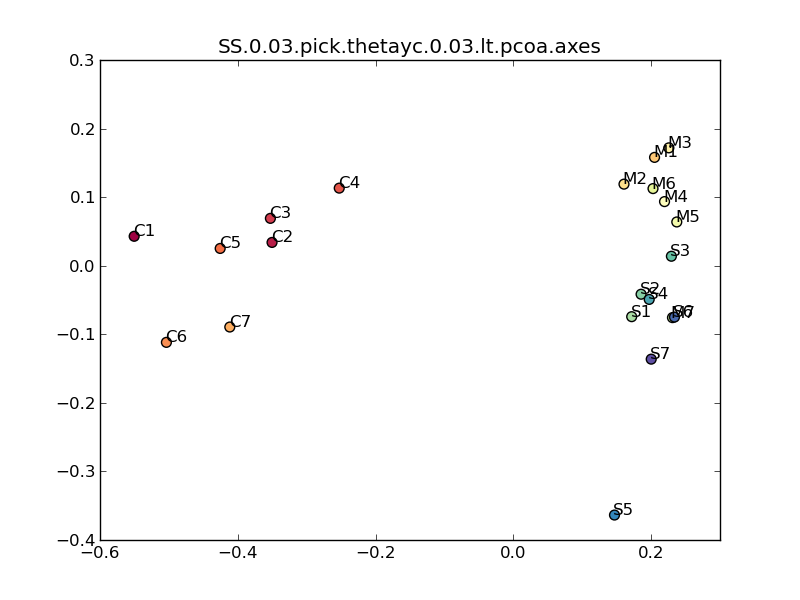
\includegraphics[width=0.8\textwidth]{figures/otu-pcoa.png}
    \caption[PCoA plot of microbial community structure using SSU rRNA gene]{PCoA plot of microbial community structure using SSU rRNA gene from shotgun metagenome. Three crops have significantly different communities (AMOVA test: $p < 0.001$) and corn is the most different.}
    \label{fig:otu-pcoa}
    \end{figure}


    \begin{figure}[tbph!]
    \centering
    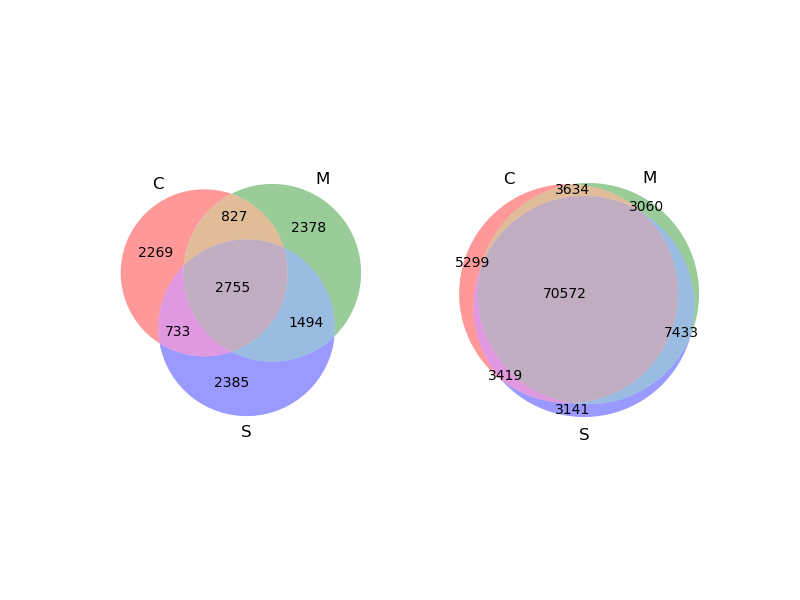
\includegraphics[width=0.8\textwidth]{figures/otu-venn}
    \caption[Venn diagram of OTUs]{Venn diagram of OTUs among rhizosphere microbial community among three crops. The one on the left does not consider abundance of OTU (unique) and the one on the right considers abundance. The shared unique OTUs is 21.5\% (left) of total but 73.1\% (right) when weighted by abundance.}
    \label{fig:otu-venn}
    \end{figure}


    \begin{figure}[tbph!]
    \centering
    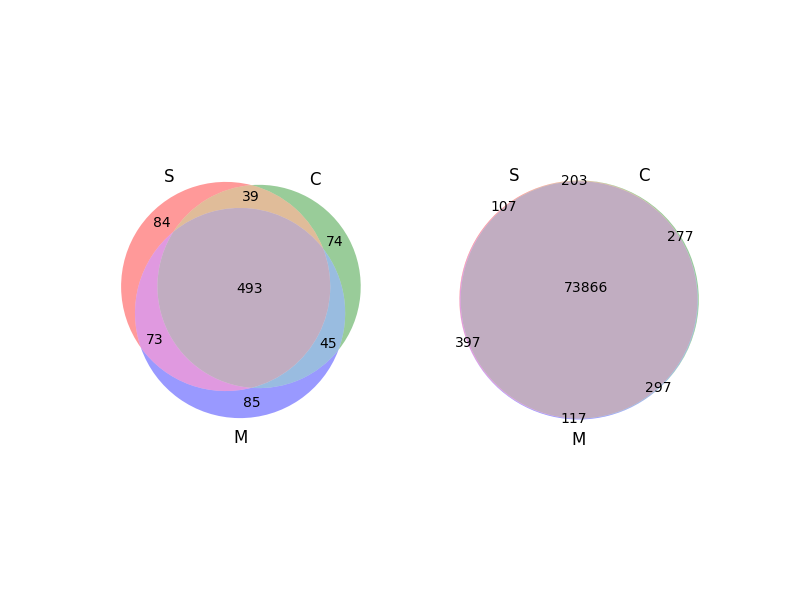
\includegraphics[width=0.8\textwidth]{figures/genus-venn}
    \caption[Venn diagram of genera]{Venn diagram of genera among rhizosphere microbial community among three crops. The one on the left does not consider abundance of OTU (unique) and the one on the right considers abundance. The shared unique OTUs is 55.2\% (left) of total but 98.1\% (right) when weighted by abundance.}
    \label{fig:genus-venn}
    \end{figure}


    \begin{figure}[tbph!]
    \centering
    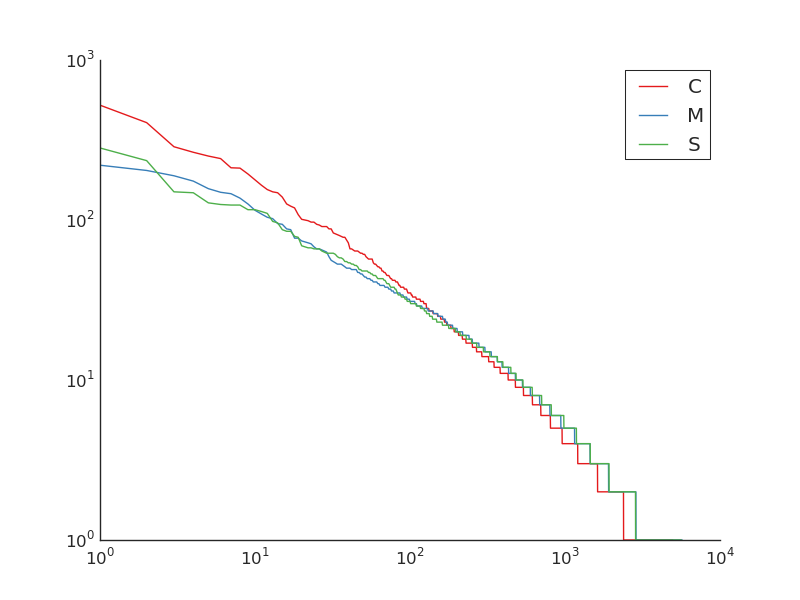
\includegraphics[width=0.8\textwidth]{figures/otu-rankabuncurve}
    \caption[Rank abundance curve]{Rank abundance curve of microbial community of corn, Miscanthus and switchgrass. Corn has the most uneven microbial community in rhizosphere.}
    \label{fig:otu-rankabuncurve}
    \end{figure}


    \begin{figure}[tbph!]
    \centering
    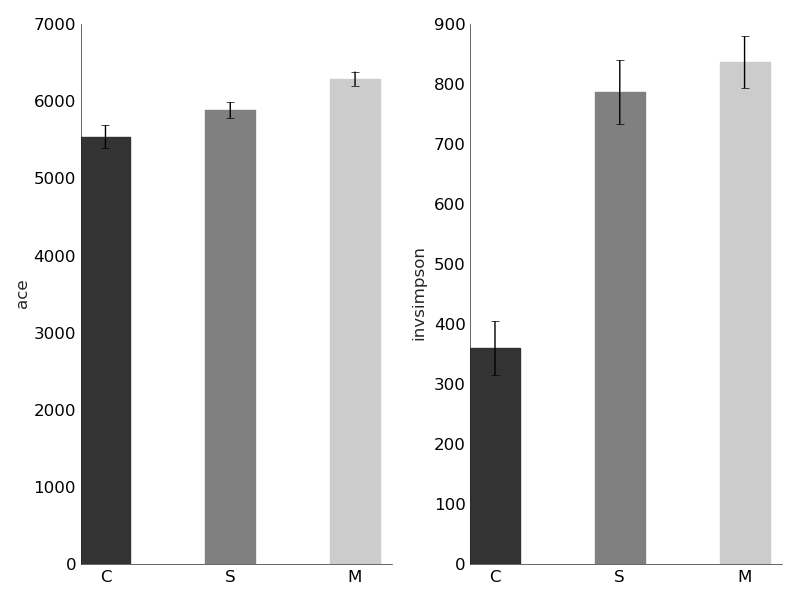
\includegraphics[width=0.8\textwidth]{figures/otu-alpha-div}
    \caption[Alpha diversity]{Alpha diversity of microbial community of three crops. Corn has lower diversity than Miscanthus and switchgrass.}
    \label{fig:otu-alpha-div}
    \end{figure}



    \begin{figure}[tbph!]
    \centering
    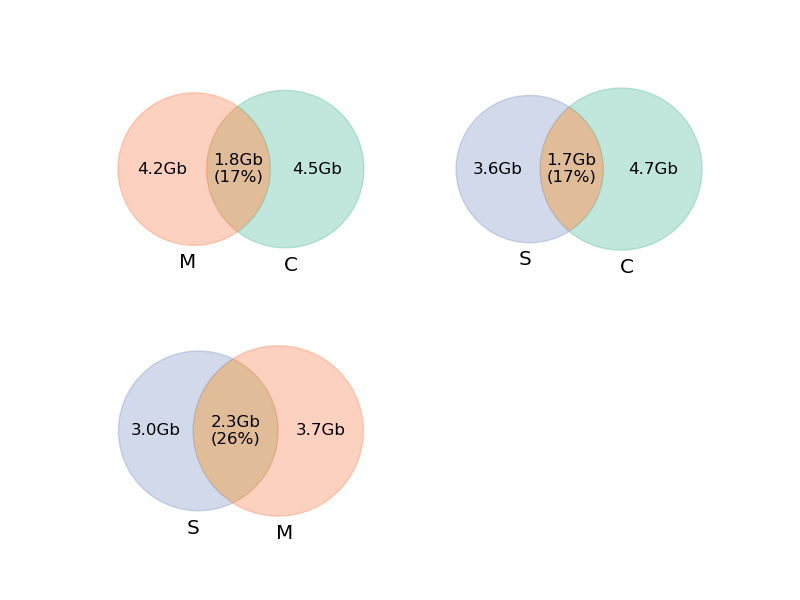
\includegraphics[width=0.8\textwidth]{figures/contig-sim-venn}
    \caption[Assembly sequence similarity]{Assembly sequence similarity among three crops. Corn is the most different.}
    \label{fig:contig-sim-venn}
    \end{figure}


    \begin{figure}[tbph!]
    \centering
    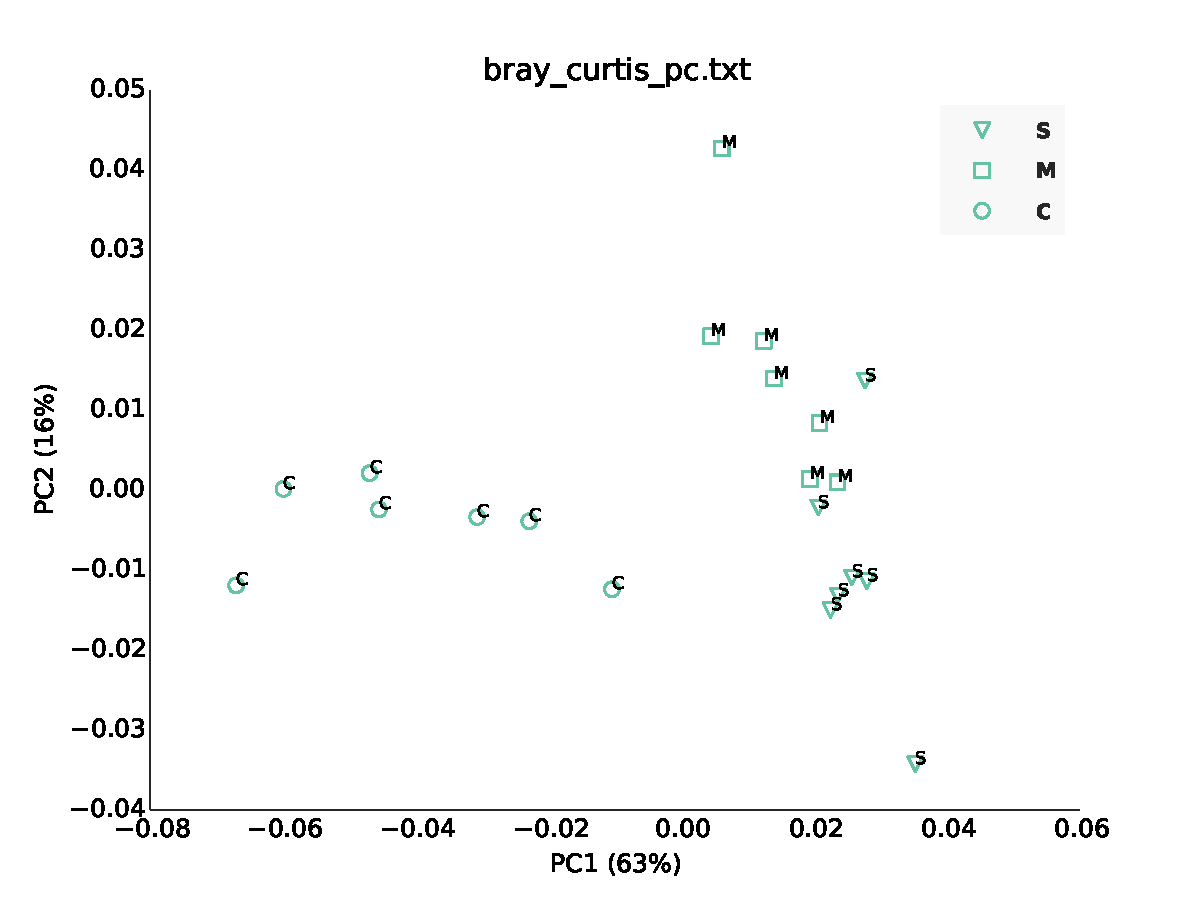
\includegraphics[width=0.8\textwidth]{figures/subsys-l3-pcoa}
    \caption[PCoA plot based on subsystem profile]{PCoA plot of subsystem level 3 function profile of three crops. The subsystems profiles are functional annotation from assemblies. Three crops have significantly different communities and corn is the most different.}
    \label{fig:subsys-l3-pcoa}
    \end{figure}

    \begin{figure}[tbph!]
    \centering
    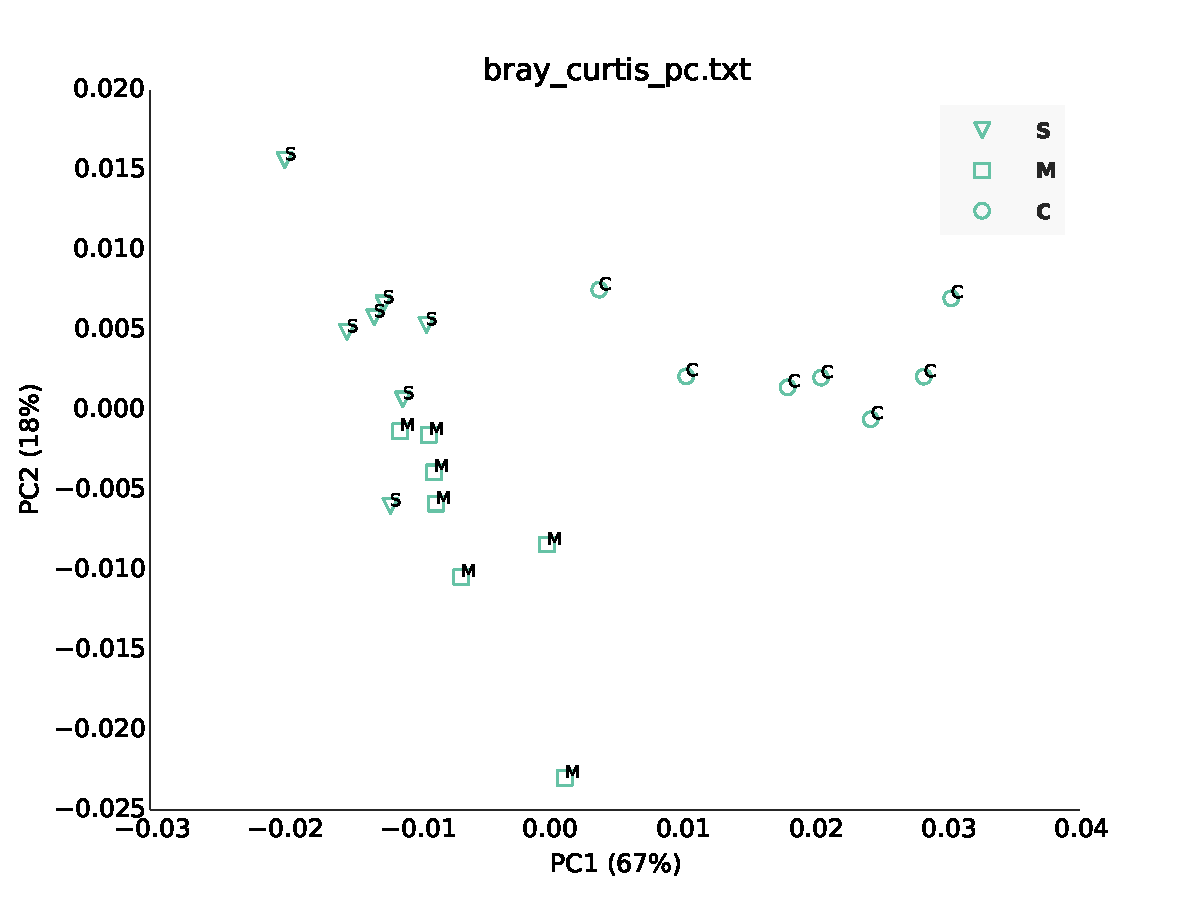
\includegraphics[width=0.8\textwidth]{figures/subsys-l1-pcoa}
    \caption[PCoA plot based on subsystem profile]{PCoA plot of subsystem level 1 function profile of three crops. The subsystems profiles are functional annotation from assemblies. Three crops have significantly different communities and corn is the most different.}
    \label{fig:subsys-l1-pcoa}
    \end{figure}


    \begin{figure}[tbph!]
    \centering
    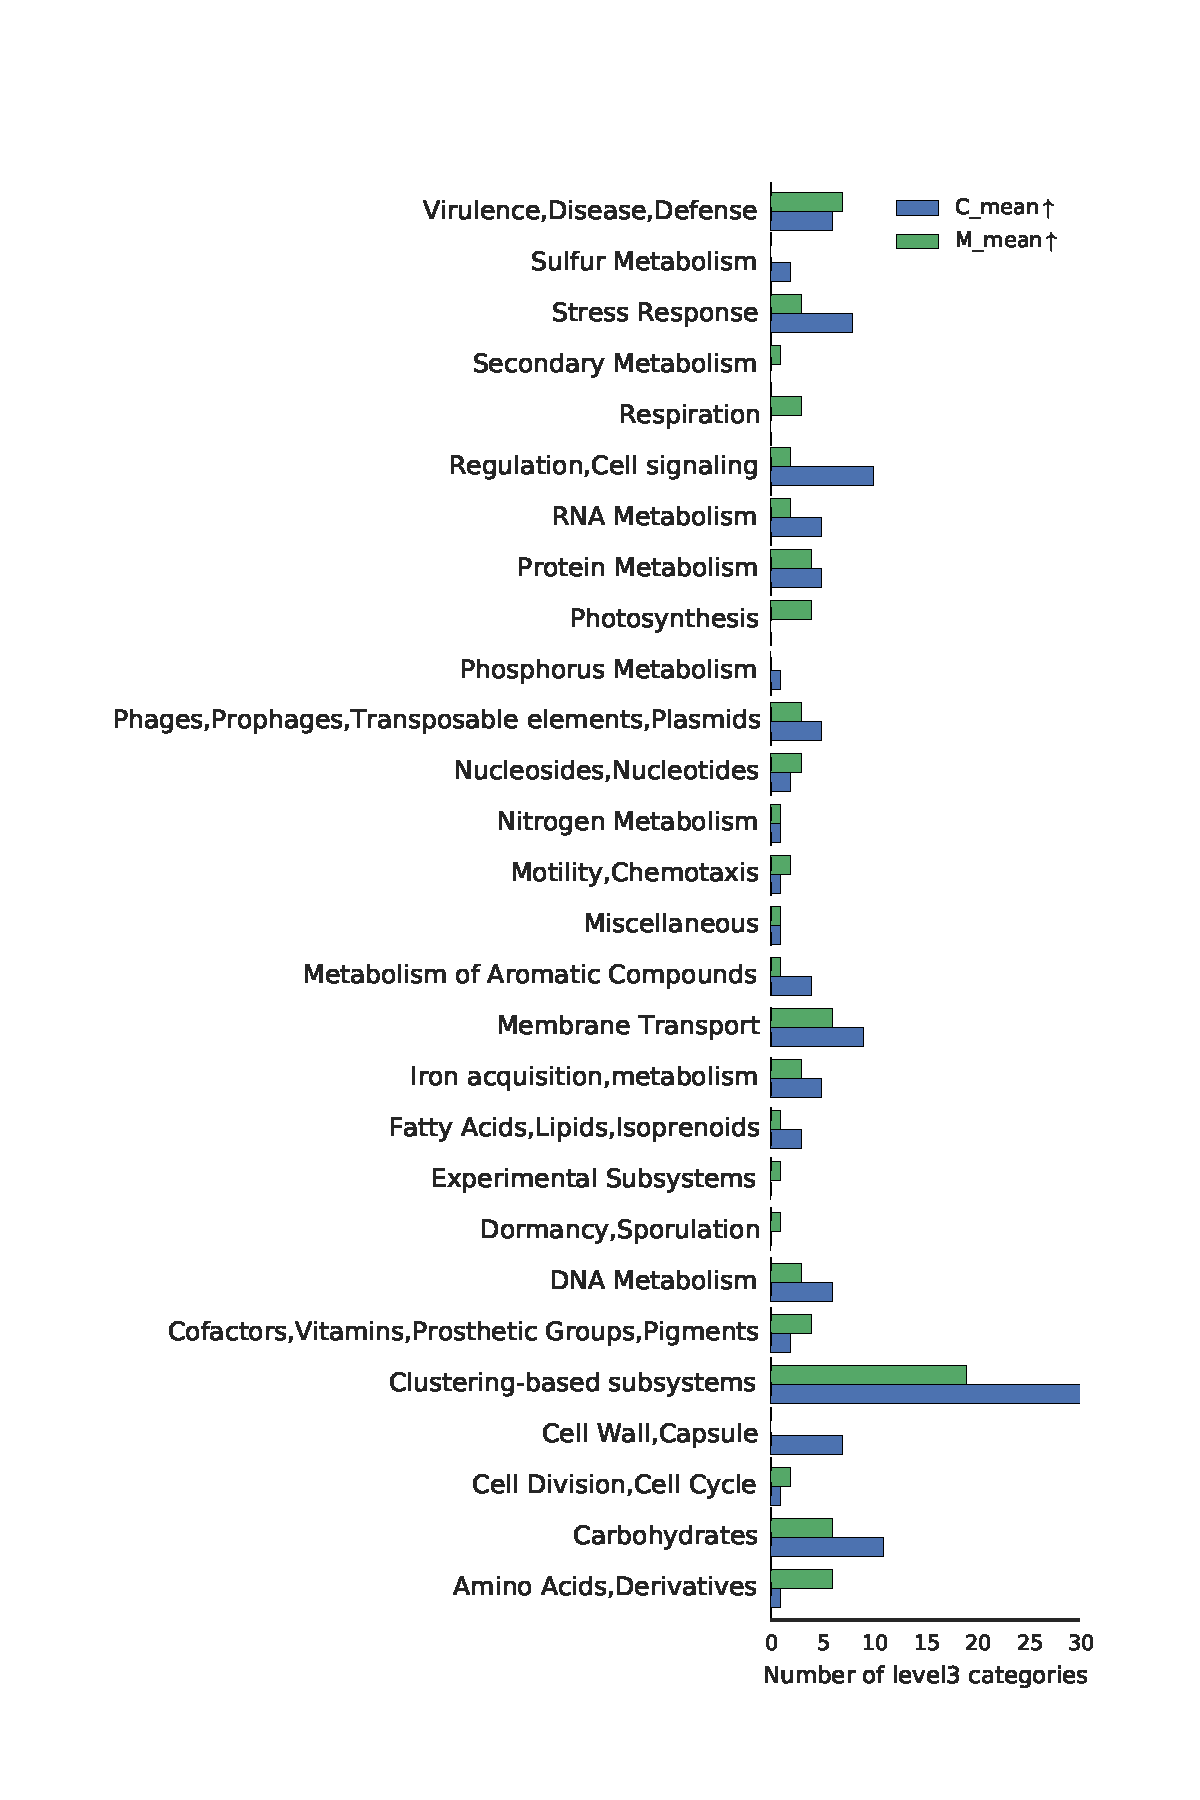
\includegraphics[width=0.8\textwidth]{figures/subsys-enrich-CvM}
    \caption[Number of pathways enriched in categories in subsystem level 1]{Number of pathways enriched (in either corn or miscanthus) in categories in subsystem level 1. ``Carbohydrate metablism'', ``Stress response'', and ``Cell wall'' categories are enriched corn, while ``Amino acid'' are enriched in Miscanthus.}
    \label{fig:subsys-enrich-CvM}
    \end{figure}



    \begin{figure}[tbph!]
    \centering
    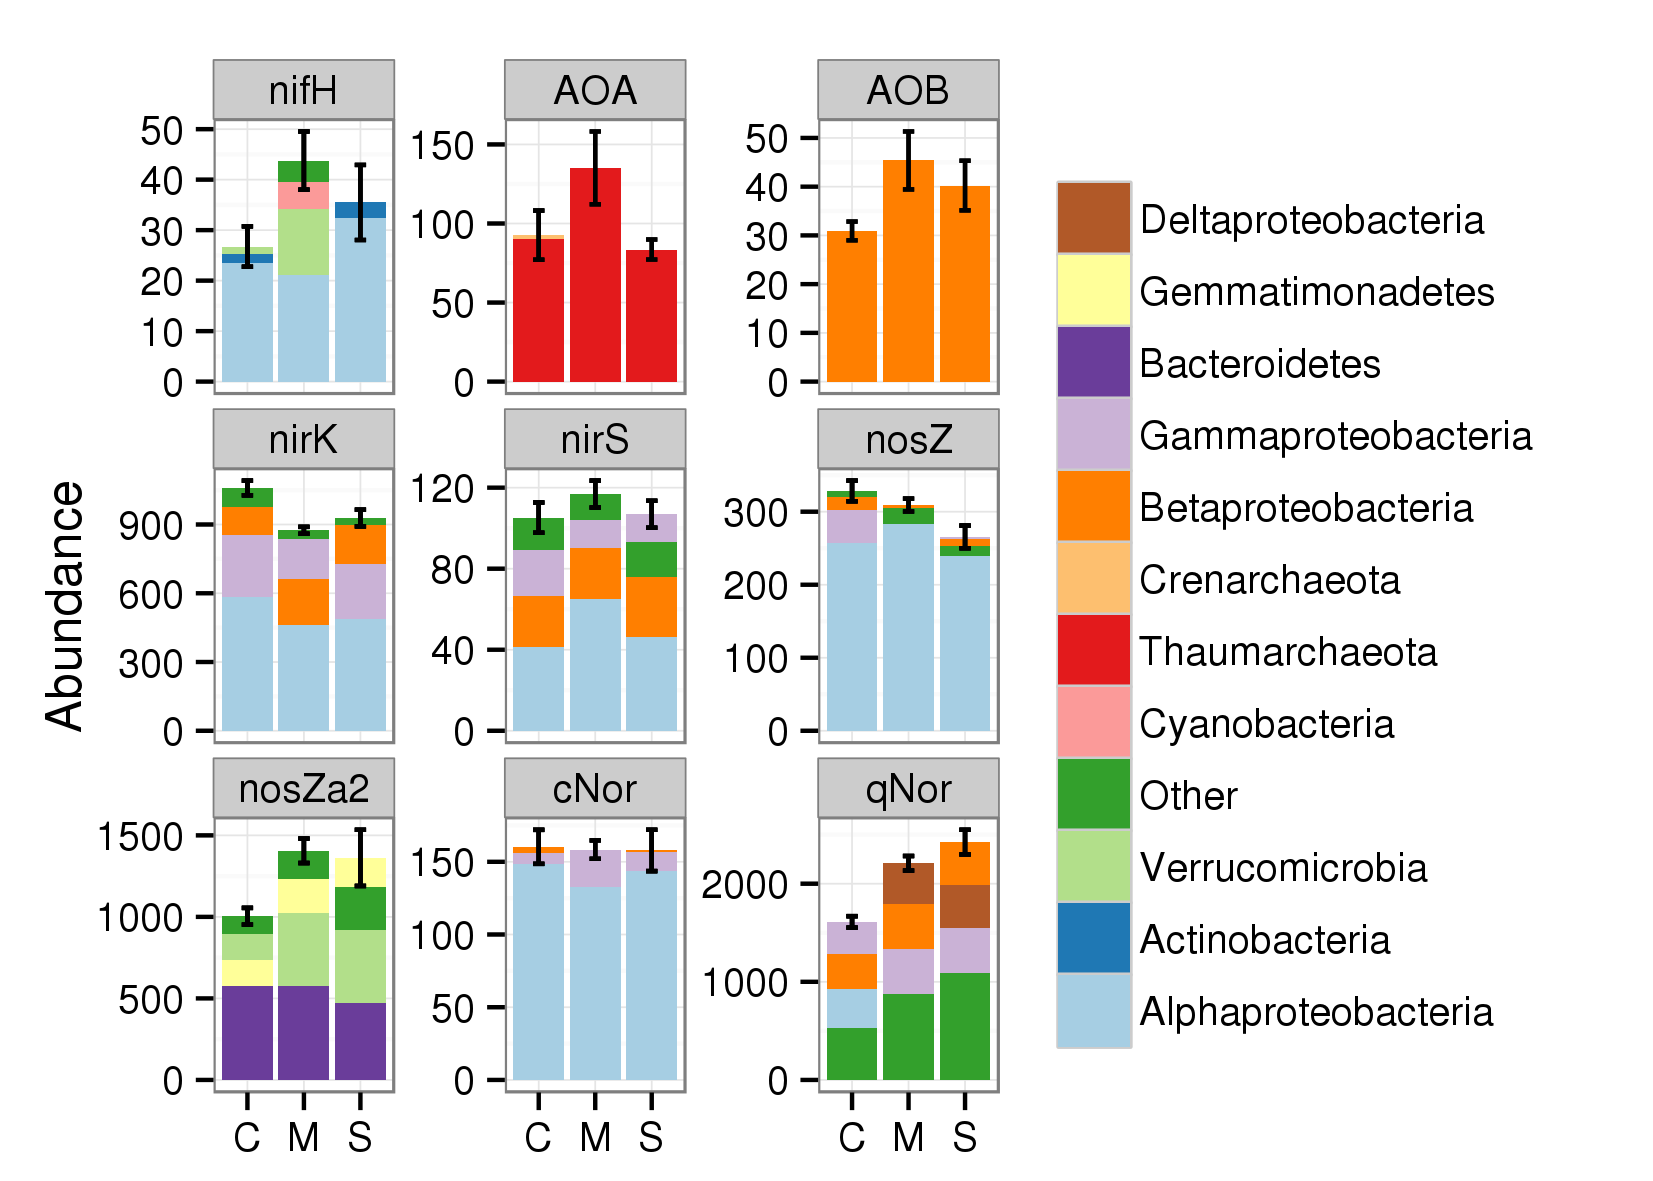
\includegraphics[width=0.8\textwidth]{figures/xander-ncycle-abun}
    \caption[Abundance and phylum level distribution of N cycle genes]{Abundance and phylum level distribution of N cycle genes. Each genes is standardized by rplB.}
    \label{fig:xander-ncycle-abun}
    \end{figure}


    \begin{figure}[tbph!]
    \centering
    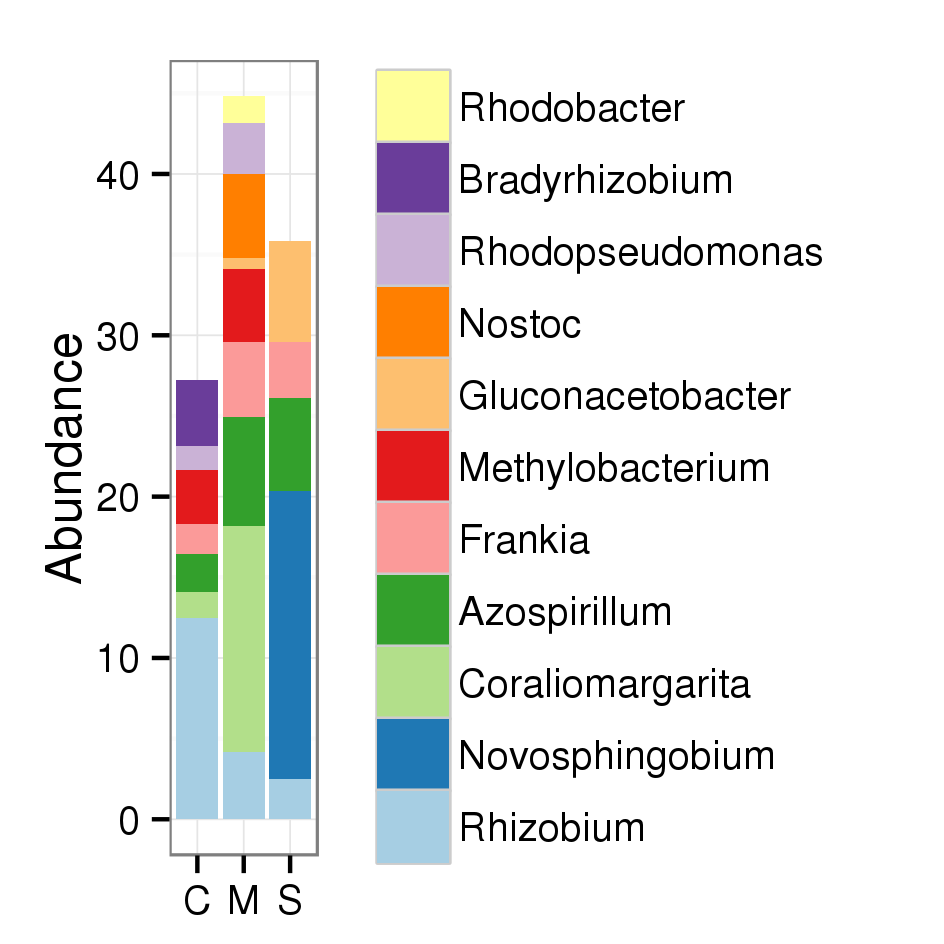
\includegraphics[width=0.8\textwidth]{figures/xander-nifH-genus}
    \caption[Abundance and genus level distribution of nifH]{Abundance and genus level distribution of nifH. Abundance is standardized by rplB. Three crops are quite different in genus composition. Miscanthus is the most abundant in nifH and has the most number of genera.}
    \label{fig:xander-nifH-genus}
    \end{figure}


    \begin{figure}[tbph!]
    \centering
    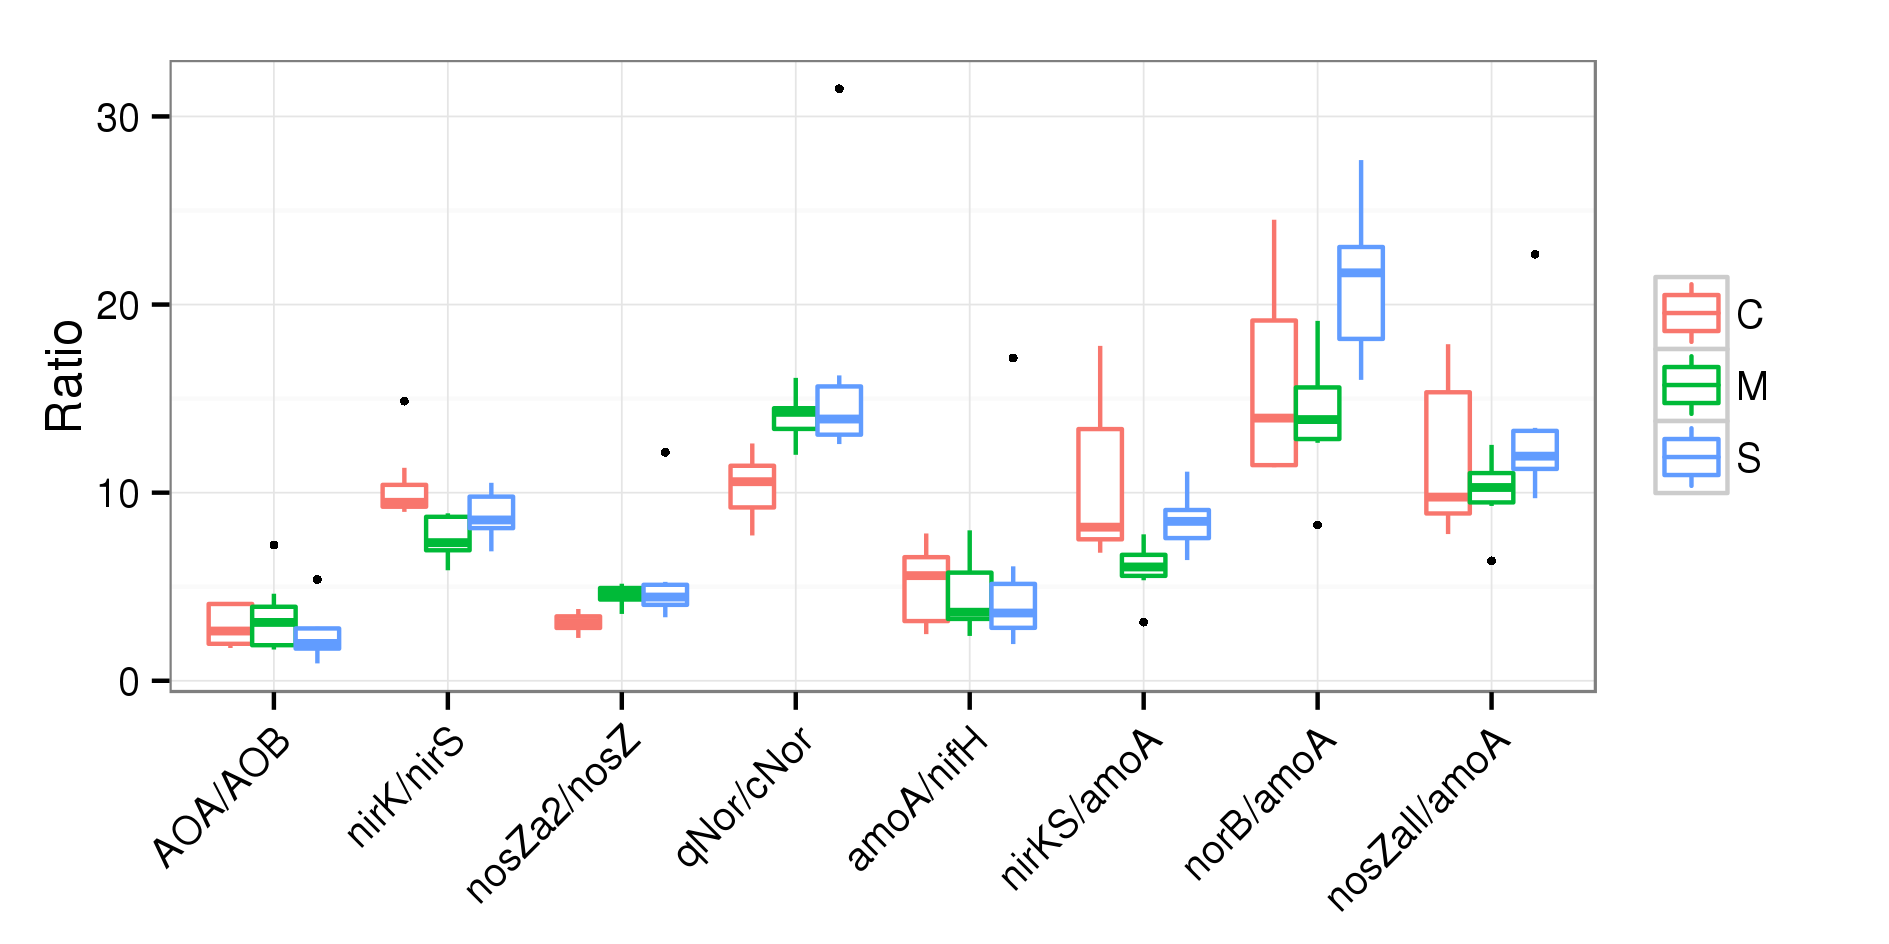
\includegraphics[width=0.8\textwidth]{figures/xander-ncycle-ratio}
    \caption[Ratios of interest related to N cycle genes]{Ratios of interest related to N cycle genes.}
    \label{fig:xander-ncycle-ratio}
    \end{figure}


\end{document}